\section*{Part 4：Stratified CV 與 Hyperparameter Selection}
\vspace{-0.5em}

\q{14}{搜尋設計。}
只使用 Dataset A 的訓練資料，透過 \metric{StratifiedKFold(5, shuffle=True, random\_state=42)} 比較 13 組超參數設定，評估指標為 \metric{f1\_macro}。kNN 與 SVM 使用 Pipeline，確保每一折的 StandardScaler 都只從該折訓練資料學習；Decision Tree 使用原始特徵。測試集不參與參數選擇。

\q{15}{各候選五折平均與母體標準差（\texttt{ddof=0}）。}
\begin{center}
\scriptsize
\rowcolors{2}{lightrow}{white}
\begin{tabular}{llrr@{\qquad}llrr@{\qquad}llrr}
\toprule
模型 & 設定 & Mean & Std & 模型 & 設定 & Mean & Std & 模型 & 設定 & Mean & Std \\
\midrule
kNN & $k=1$ & .9434 & .0201 & Tree & $d=2$ & .9275 & .0202 & SVM & $C=.1$ & .9377 & .0180 \\
kNN & $k=3$ & .9596 & .0096 & Tree & $d=3$ & .9204 & .0091 & SVM & $C=1$ & .9669 & .0160 \\
kNN & $k=5$ & .9598 & .0118 & Tree & $d=5$ & .9188 & .0123 & SVM & $C=10$ & .9671 & .0136 \\
kNN & $k=9$ & .9620 & .0158 & Tree & $d=10$ & .9119 & .0190 & & & & \\
kNN & $k=15$ & .9570 & .0180 & Tree & $d=$None & .9119 & .0190 & & & & \\
\bottomrule
\end{tabular}
\end{center}
每一列另保留五個 fold 原始分數於 \metric{cv\_search\_a.csv}。

\begin{center}
\begin{minipage}{0.90\linewidth}
\centering
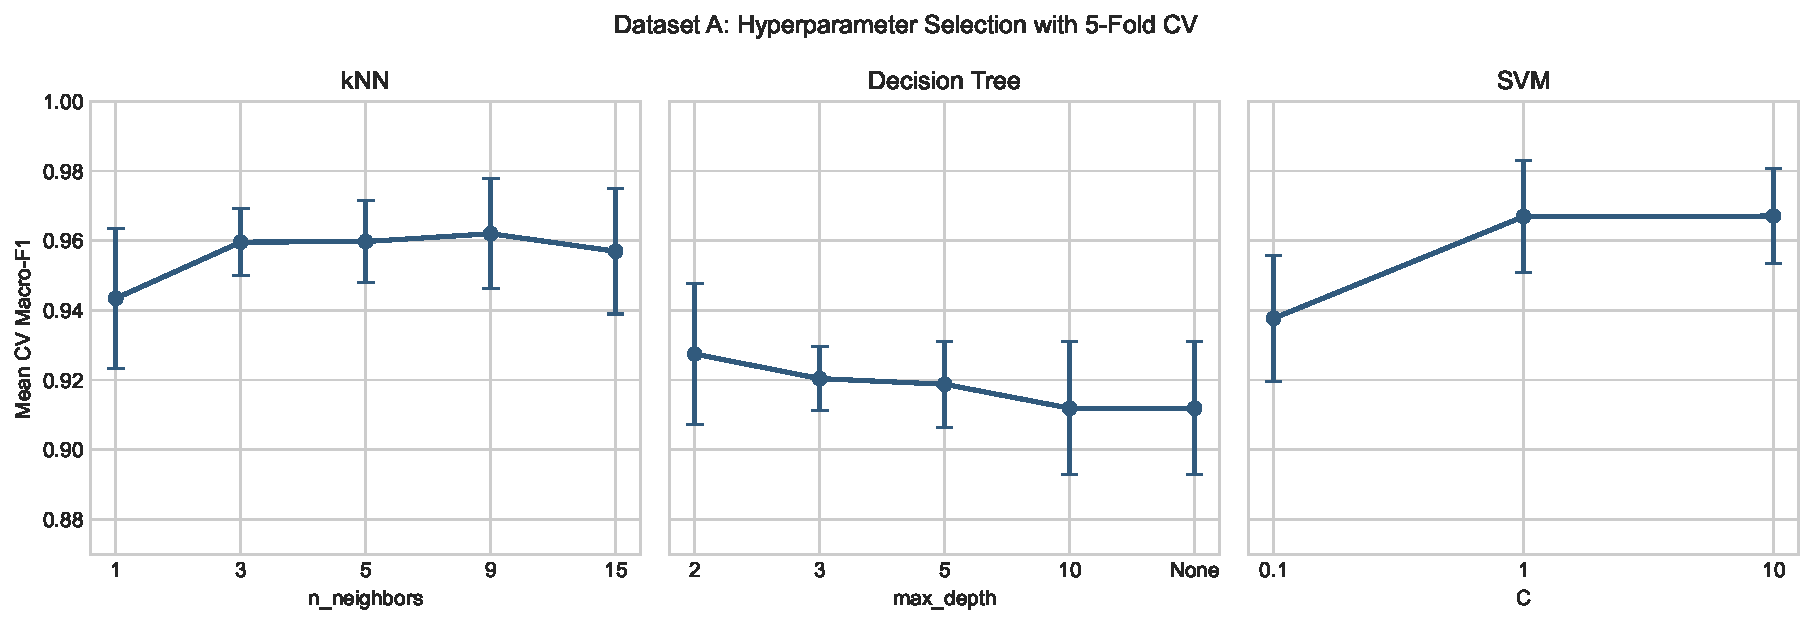
\includegraphics[width=0.92\linewidth]{cv_hyperparameters.pdf}
\par\small Figure 2：候選參數的 training-only CV Macro-F1；error bars 為五折母體標準差。
\end{minipage}
\end{center}

\q{16}{選定設定。}
主要依照平均 Macro-F1 選擇參數，若分數相同，則參考標準差與模型複雜度：kNN 選 $k=9$（.9620$\pm$.0158）、Tree 選 depth 2（.9275$\pm$.0202）、SVM 選 $C=10$（.9671$\pm$.0136）。SVM 的 $C=10$ 與 $C=1$ 平均分數非常接近，但前者的標準差也較小，因此仍選擇 $C=10$。上述選擇均依據交叉驗證結果，未參考測試集分數。

\q{17}{敏感度與「最高 training performance」問題。}
比較各候選設定的平均 Macro-F1，kNN 的最大差距為 0.0186、Decision Tree 為 0.0156、SVM 為 0.0294，因此在本次設定範圍內，SVM 對參數變化最敏感。訓練分數高也不代表泛化效果最好。例如未限制深度的決策樹平均僅 .9119，低於深度 2 的 .9275，顯示模型複雜度增加未必帶來更好的交叉驗證表現。

\q{18}{設定鎖定後的固定 test 一次評估。}
\begin{center}
\compacttable
\begin{tabular}{llrrrrrr}
\toprule
模型 & CV 選定 & Raw Acc. & Raw F1 & Scaled Acc. & Scaled F1 & Final Acc. & Final F1 \\
\midrule
kNN & $k=9$ & .9123 & .9066 & .9561 & .9526 & .9737 & .9713 \\
Tree & $d=2$ & .9123 & .9075 & .9123 & .9075 & .8947 & .8907 \\
SVM & $C=10$ & .9298 & .9230 & .9825 & .9812 & .9737 & .9719 \\
\bottomrule
\end{tabular}
\end{center}
kNN 的提升主要先來自標準化（Macro-F1 +.0460），再經交叉驗證選參提高到 .9713。SVM 在 $C=1$ 且標準化時的測試分數為 .9812，改用交叉驗證選出的 $C=10$ 後則是 .9719；雖然略低，仍不應根據測試結果回頭改選參數。Decision Tree 選擇深度 2 後，測試 Macro-F1 也降至 .8907。這些結果提醒我們：交叉驗證選出的參數不保證在單次測試切分中一定進步。
